\documentclass[t, 9pt, aspectratio=169]{beamer}
\usetheme{phw}

\title{Long Time Logging}
\subtitle{}
\author{Adrian Dumitrescu}
\institute{ThermoFisher Scientific}
\date{June 23rd, 2022}

\begin{document}
    \begin{frame}
        \titlepage
    \end{frame}

    \begin{frame}
        \frametitle{Outline}
        \tableofcontents
    \end{frame}

    \section{Round Robin Database}
    \subsection{Data Collection and Storage}

    \begin{frame}{Round Robin Database}{Data Collection and Storage}
        \begin{itemize}
            \item Collects data from multiple \highlight{data sources}
            \begin{itemize}
                \item each data source has a name and defines a specific data sample frequency (rate) e.g. RPM value once per second, temperature once every 5 seconds
            \end{itemize}
            \item Stores collected data in multiple \highlight{archives}
            \begin{itemize}
                \item archives are defined at database level
                \item each archive defines a data sample frequency (rate) e.g. one value every second, every minute, every hour
                \item also, the last value\footnotemark of each data source is available
            \end{itemize}
            \footnotetext{not same as last stored value}
        \end{itemize}
        \begin{figure}
            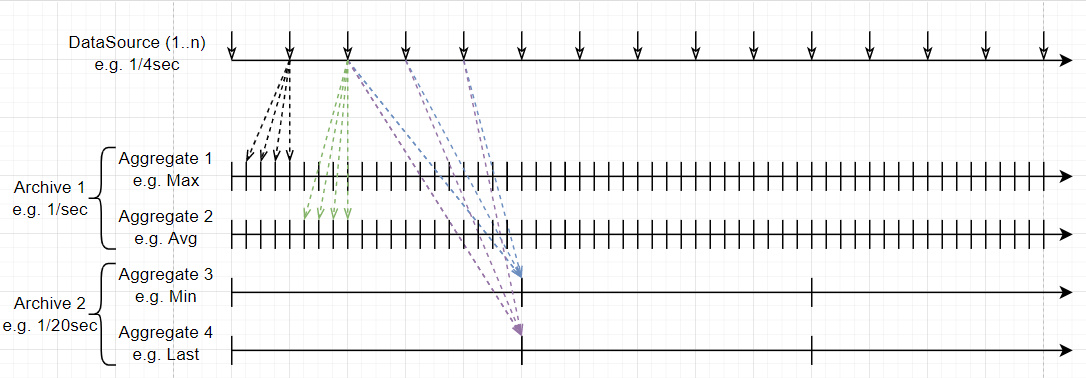
\includegraphics[scale=0.35]{rrdb-structure.jpg}
        \end{figure}
    \end{frame}

    \subsection{Aggregation/Resampling}

    \begin{frame}{Round Robin Database}{Aggregation/Resampling}
        \begin{figure}
            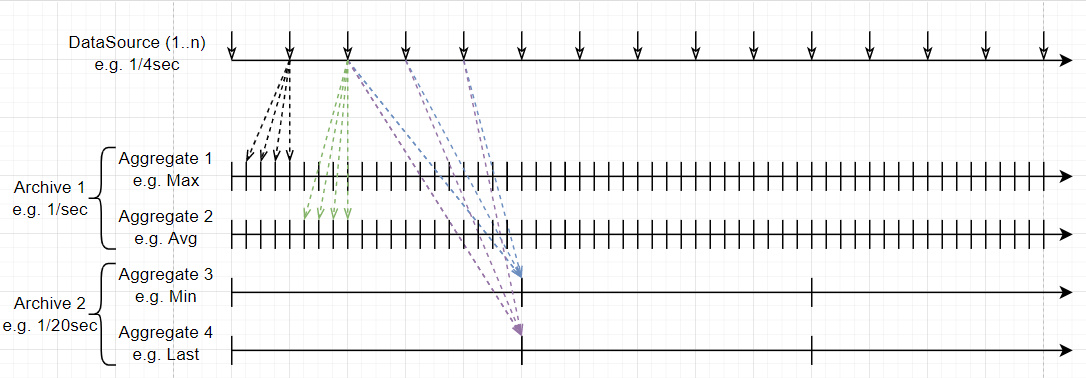
\includegraphics[scale=0.35]{rrdb-structure.jpg}
        \end{figure}
        \begin{itemize}
            \item Mismatch between the sampling frequencies of each data source and of each archive
            \item Resampling needed before storing: \highlight{aggregation}
            \item Each data source defines 0 or more aggregations (one of: Min, Max, Average, Last)
        \end{itemize}
    \end{frame}

    \subsection{Trivia}

    \begin{frame}{Round Robin Database}{Trivia}
        The current database is setup with 3 archives containing data samples for
        \begin{itemize}
            \item every second for 72 hours
            \item every minute for 60 days
            \item every hour for about 9.75 years\footnotemark
        \end{itemize}
        \footnotetext[1]{probably a mistake; likely intended to be 10 years}
    \end{frame}

    \section{Data Aggregation}
    \subsection{Supersampling}

    \begin{frame}{Data Aggregation}{Supersampling}
        \vspace{-1cm}
        \begin{figure}
            \hspace*{-1cm}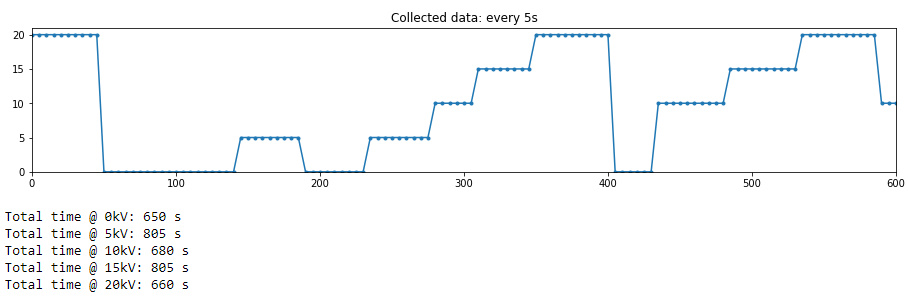
\includegraphics[scale=0.5]{collected-data-5s.jpg}
            \hspace*{-1cm}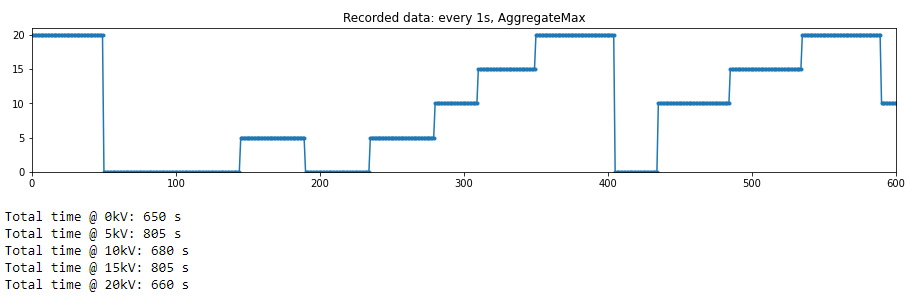
\includegraphics[scale=0.5]{aggregate-max-1s.jpg}
        \end{figure}
    \end{frame}

    \subsection{Subsampling}

    \begin{frame}{Data Aggregation}{Subsampling}
        \vspace{-1cm}
        \begin{figure}
            \hspace*{-1cm}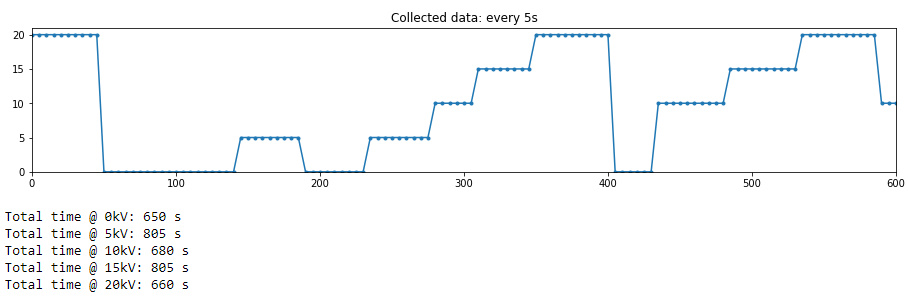
\includegraphics[scale=0.5]{collected-data-5s.jpg}
            \hspace*{-1cm}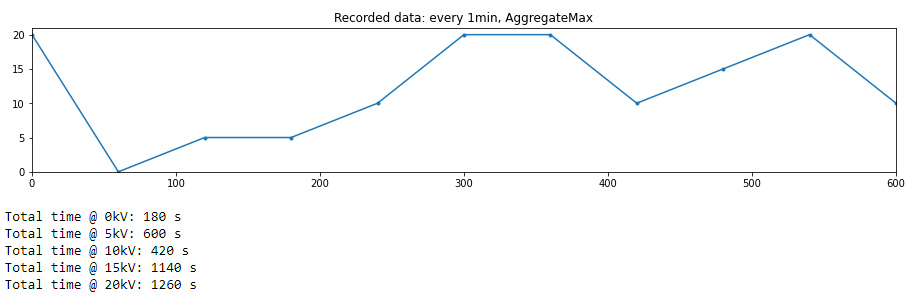
\includegraphics[scale=0.5]{aggregate-max-1min.jpg}
        \end{figure}
    \end{frame}

    \begin{frame}{Data Aggregation}{Subsampling}
        \vspace{-1cm}
        \begin{figure}
            \hspace*{-1cm}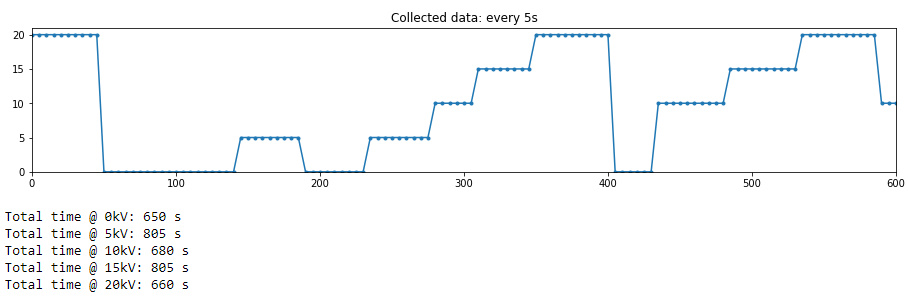
\includegraphics[scale=0.5]{collected-data-5s.jpg}
            \hspace*{-1cm}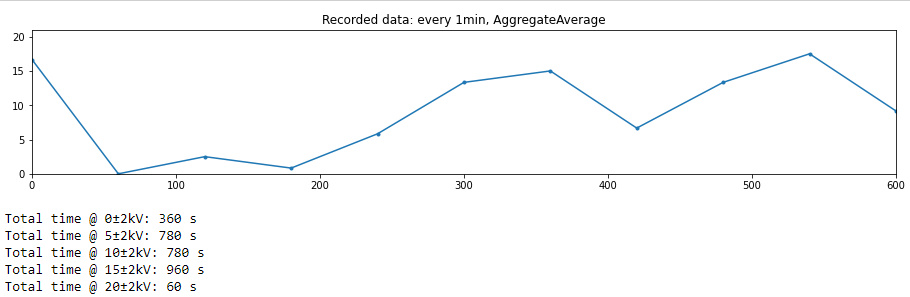
\includegraphics[scale=0.5]{aggregate-avg-1min.jpg}
        \end{figure}
    \end{frame}

    \section{Round Robin Database}
    \subsection{Limitations}
    
    \begin{frame}{Data Aggregation}{Limitations}
        \begin{itemize}
            \item Fixed size database\footnotemark, long term history of value evolution
            \item Total size (hence number of data sources and aggregates) to be kept in check
            \item Re-(sub-)sampling (i.e. low resolution of sampling) makes extracting totals difficult or unfeasible
            \item Totals and counters \highlight{may but don't need to} be part of the long term logging; they could be recorded in other forms of persistent storage
        \end{itemize}
        \footnotetext{for one aggregation of one data source}
    \end{frame}

    \section{Operational Values}
    \subsection{Which Values to Log?}
    
    \begin{frame}{Operational Values}{Which Values to Log?}
        \begin{itemize}
            \item Define a list or a method to identify the values (and aggregations) to be recorded in the long term database
            \begin{itemize}
                \item There seems to be some consensus that all "sensible" TAD values should be logged
                \begin{itemize}
                    \item not: strings, versions, video ADCs etc.
                    \item boolean or enum-like values might or might not be useful when aggregated
                \end{itemize}
                \item There is a proposal of adding other parameters but they are mostly just overall totals or counters (like total distance travelled by stage axes or number of valve actions)
                \item Stigmation and source tilt (X and Y) history could qualify, but not sure how the loss of resolution would impact them
            \end{itemize}
        \end{itemize}
    \end{frame}

    \begin{frame}{Operational Values}{In TestUI}
        \vspace*{-1cm}
        \begin{figure}
            \hspace*{-0.8cm}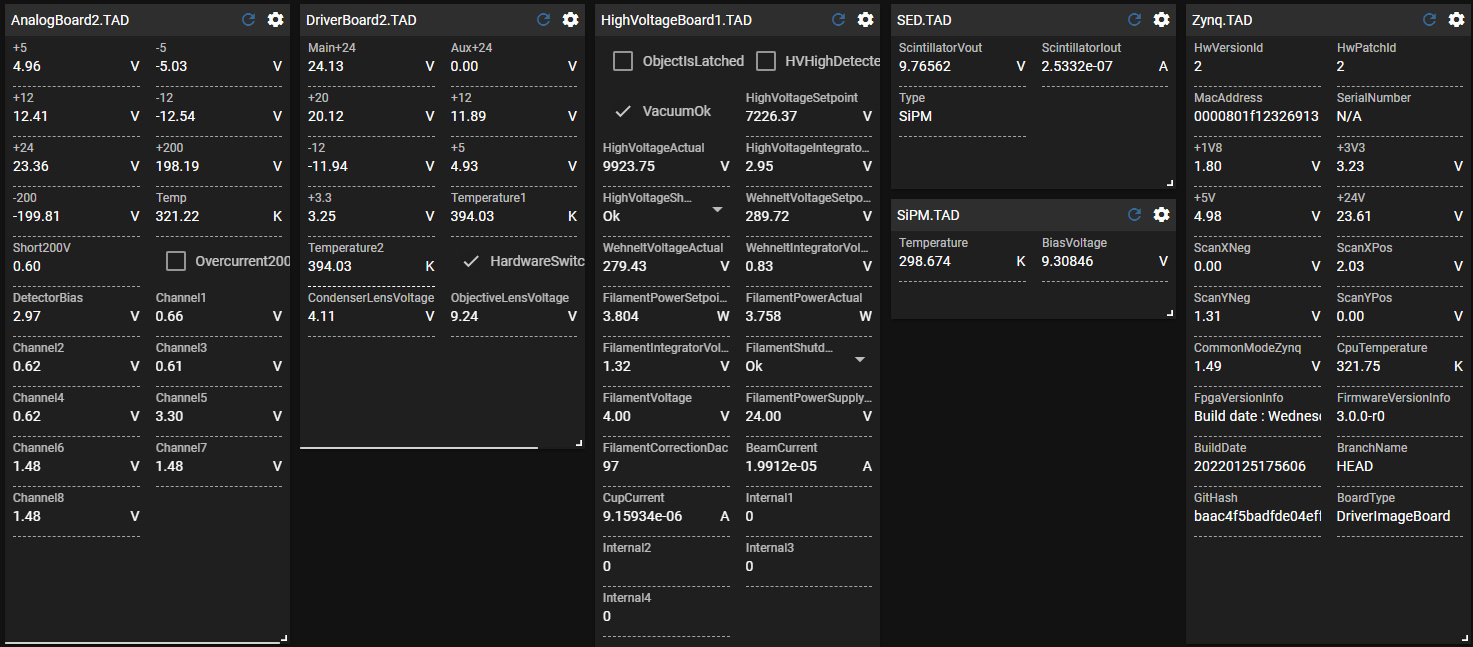
\includegraphics[scale=0.37]{tad-accessors-xl2.jpg}
        \end{figure}
        Not all values can or should be logged.
    \end{frame}

    \begin{frame}{Operational Values}{In PhenomServiceTool}
        \vspace*{-1cm}
        \begin{figure}
            \hspace*{0.5cm}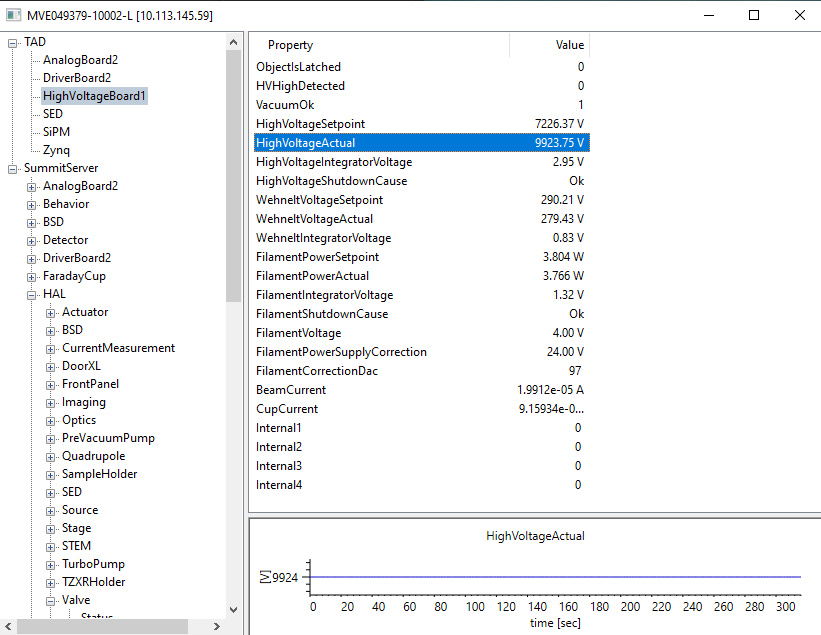
\includegraphics[scale=0.47]{tad-accessors-service-tool.jpg}
        \end{figure}
    \end{frame}

    \subsection{Plan}

    \begin{frame}{Operational Values}{Plan}
        \begin{itemize}
            \item Add all "sensible" TAD values and the two already requested (Stigmation and SourceTilt)
            \item Decide on how to handle totals and counters
            \item Collect input from R\&D, Service, Apps over which other values to add
            \item Critically select which to add and which not, based on maximizing the "usefulness"
        \end{itemize}
    \end{frame}

    \begin{frame}{Operational Values}{In SysInfoViewer}
        \vspace*{-0.8cm}
        \begin{figure}
            \hspace*{-0.7cm}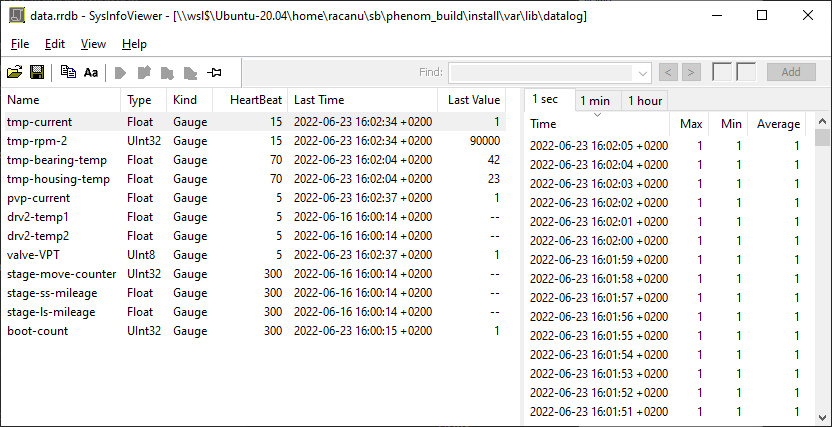
\includegraphics[scale=0.5]{rrdb-in-sysinfoviewer.jpg}
        \end{figure}
    \end{frame}

    \section{Questions and Discussions}

    \begin{frame}{Questions and Discussions}
    \end{frame}
\end{document}